\chapter{Modelling a Database for Dynamic Multimedia Data}
\label{chapter:system_model}

\section{Generalized Distance Based Operations}

Starting with the metric space model~\cite{Zezula:2006similarity} for similarity search presented in \Cref{chapter:theory_multimedia_analysis_and_retrieval}, we propose to extend the notion of proximity-based similarity search to that of a more general \emph{proximity based query} following \cref{definition:pbq}.

\begin{definition}[label=definition:pbq]{Proximity Based Query}{}
    Any database query operation on relation $\mathcal{R}$ that relies on the evaluation of a distance function $\delta(a_{i}, q)$ that calculates the distance between an attribute $a_{i} \in \mathcal{D}_q$ and some query $q \in \mathcal{D}_q$ given $\mathcal{D}_q \in \mathtt{SCH}(\mathcal{R})$ and distance function $\delta: \mathcal{D}_q \times \mathcal{D}_q \rightarrow \mathbb{R}$, is called a \emph{proximity based query}. We call $q$ the \emph{query} and $a_i$ the \emph{probing attribute} both sharing the same \emph{query data domain} $\mathcal{D}_q$.
\end{definition}

It is important to note, that \cref{definition:pbq} simply requires a notion of proximity between some attribute and a query to be obtained by evaluating some distance function. The definition does not make any assumption as to what data domains $\mathcal{D}_q$ query and probing attribute belong to nor how the distance is being used within the query, once it has been obtained. 

We observe, that similarity search falls into the broader category of a proximity based queries, wherein the distance is used to rank the relation and subsequently limit its cardinality. Additionally, proximity based queries include operations such as evaluating a distance function followed by some filtering or grouping based on the computed value, i.e, we are not limited to mere search.

\subsection{Revisiting Distance Computation}

Since the choice of the distance function $\delta$ is a crucial part of any proximity based query, it is worth revisiting its definition. Again, starting with the metric space modell~\cite{Zezula:2006similarity}, we identify the following (implicit) constraints with respect to the distance function:

\begin{enumerate}
    \item The codomain (i.e., the output) of the distance function $\delta$ is assumed to be $\mathbb{R}_{\geq 0}$, hence, the generated distance value is a positive, real number.
    \item The domain (i.e., the input) of the distance function $\delta$ is assumed to be $\mathbb{R}^{dim} \times \mathbb{R}^{dim}$, hence, restricted to real-valued vectors and the distance function is assumed to be a binary function.
    \item $(\mathcal{D}_q,\delta)$ are supposed to constitute a metric, thus satisfying the non-negativity, identity of indiscernibles, symmetry and subadditivity properties.
\end{enumerate}

Upon closer examination, one can see that there is good reason to assume the codomain of $\delta$ to lie in $\mathbb{R}$. On the one hand, it is obviously convenient both for the underlying mathematics as well as from a programming prespective. More importantly, however, real numbers -- unlike, for example, complex numbers or vectors -- come with a natural, total ordering, which is required for the sorting that is part of many proximity based queries. If, however, we turn to \cref{example:mrf}, we realise that it is not reasonable to impose a restriction of the domain of the distance function to $\mathbb{R}^{dim}$ with $dim \in \mathbb{N^{+}}$

\begin{example}[label=example:mrf]{Maximum Inner Product Search (MIPS) for MRF}{}
    In MRF (see \cref{section:application_mrf}), we try to obtain the signal vector $a_{i \in \mathbb{N}} \in \mathcal{D}_q \subset \mathbb{C}^{dim}$ so that it maximizes the inner product to a query vector $q \in \mathbb{C}^{dim}$. In this case, the distance function $\delta$ has the form $\delta \colon \mathbb{C}^{dim} \times \mathbb{C}^{dim} \to \mathbb{R}_{\geq 0}$. Hence, the domain of $\delta$ is a complex vector space.
\end{example}

Obviously, this limitation of the definition of $\delta$ can be easily remediated simply by extending the set of supported data domains $\mathbb{D}$ by $\mathbb{C}^{dim}$ similarily to how we did for $\mathbb{R}^{dim}$ as proposed by \cite{Giangreco:2018thesis}. Nevertheless, we have to acknowledge, that the text-book definition of a distance function is obviously too limited for some real-world applications, and that the query and probing arguments of a distance function could be any type of value supported by the database management system. Another example could be the \emph{Levenshtein distance}~\cite{Levensthtein:1965Binary} -- often used in computer linguistics -- which is a distance metric on string values.

If now in addition, we consider \cref{example:svmdistance}, we see that restricting oneself to binary functions is also too limiting when considering practical scenarios.

\begin{example}[label=example:svmdistance]{Distance Between a Vector and a Hyperplane}{}
    To find positive and negative examples $a_{i} \in \mathcal{D}_q \subset \mathbb{R}^{dim}$ given a linear classifier, e.g., provided by a SVM, we evaluate the distances between the attributes and a (query-)hyperplane described as $\mathbf{q}^T\mathbf{x} - b = 0$ with $\mathbf{q},\mathbf{x} \in \mathbb{R}^{dim}$ and $b \in \mathbb{R}$. The distance function is then given by:

    \begin{equation}
        \delta (\mathbf{a}_i, \mathbf{q}, b) = \frac{\left\|\mathbf{q}^T \mathbf{a_i} + b \right\|}{\left\|\mathbf{q}\right\|}
    \end{equation}
    
    $\delta$ now has the form $\delta \colon \mathbb{R}^{dim} \times \mathbb{R}^{dim} \times \mathbb{R} \to \mathbb{R}$. Hence, $\delta$ is no longer a binary but a ternay function with arguments $\mathbf{a_{i}}$, $\mathbf{q}$ and $b$. Furthermore, the distance may take negative values depending on whether a result is considered a positive or negative example.
\end{example}


Again, we are confronted with an example that violates the text-book definition of a distance function. While the idealized idea that distance functions used in proximity based queries must always constitute a metric on some real-valued vector space may be very common~\cite{Zezula:2006similarity}, we see in practice that this assumption is often violated~\cite{Bernhauer:2019Nonmetric} \todo{More examples} and that many functions used to calculate proximity between objects, are not actual metrics. Even though, this can be a disadvantage when considering high-dimensional index structures that exploit the geometric properties of metric functions, it is obvious that such functions exist and must thus be considered in any generalized database application supporting proximity based queries. 

To summarize, we now find ourselves in the position where, on the one hand, we require a proper definition of what is considered to be a valid distance function so as to be able to efficiently plan and execute queries, while on the other hand keeping that definition open enough to accomodate the many different, practical considerations.

In order to address the aforementioned limitations while still accomodating classical, metric distance functions and the need to be able to plan query execution, we propose the extension of a the distance function to the more general notion of a \emph{Distance Function Class (DFC)} following \cref{definition:dfc}.

\begin{definition}[label=definition:dfc]{Distance Function Classes (DFC)}{}
    A \emph{Distance Function Class (DFC)} $\hat{\delta} \colon \mathcal{D}_q \times \mathcal{D}_q \times \mathcal{D}_{1} ... \times \mathcal{D}_{n} \to \mathbb{R}$ is an n-ary but at least binary function $\hat{\delta}(a,q,s_1,...,s_n)$ that outputs a distance $d \in \mathbb{R}$ between a probing argument $a \in \mathcal{D}_q \subset \mathcal{R}$ and a query argument $q \in \mathcal{D}_q$ using a defined number of \emph{support arguments} $s_{k \in \mathbb{N}}$ from any of the data domains in $\mathbb{D}$.
\end{definition}

As a convention for notation, the probing argument $a$ of a DFC $\hat{\delta}(a,q,s_1,...,s_n)$ will always come first, followed by the query argument $q$, again followed by its support arguments $s_k$ in no particular order. 

With the idea of a DFC in mind, we can start to reason about their properties in the broader context of database operations in general and proximity based queries in particular:

\begin{description}

    \item[DFC and Execution Plans] In extension to \cref{definition:pbq}, we see that any execution plan for a database query that involves the evaluation of a DFC falls into the category of a proximity based query.

    \item[Purity] Since the purpose of a DFC is to quantify proximity between a probing argument $a$ and a query argument $q$, we require that $a, q \in \mathcal{D}_q$, i.e., both arguments must belong to the same data domain $\mathcal{D}_q \in \mathbb{D}$ for a given DFC.

    \item[Definition] A $N$-ary DFC is uniquely defined by its \emph{signature}, a ($N+1$)-tuple specifying the name of the DFC and the data domains $\mathcal{D}_i$ of the arguments it can accept as defined in \cref{equation:dfc_signature}. 

    \item[Implementation] In the context a concrete execution plan, we require the query argument $q$ and the support arguments $s_i$ for a DFC to remain constant. Hence, irrespective of the arity of the DFC, the \emph{implementation} $\delta$ of DFC $\hat{\delta}$ is always a unary function with signature ($\mathtt{NAME}, \mathcal{D}_q$), i.e., \cref{equation:dfc_implementation} holds.
\end{description}

From the perspective of the database management system, DFCs represent a family of higher-order functions\footnote{In a real-world system, available DFCs described by their signature could be stored in a global \emph{function registry} from which they can be obtained during query planning (see \cref{chapter:cottontaildb}).} that in turn parametrize unary functions using the query $q$ and support arguments $s_k$. Implementing a DFC in essence means chosing values for $q$ and $s_k$ in the context of a query. The implementation requirement enshrines the fact that for a proximity based query, altering $q$ and $s_k$ alters the executed query, which is why for a given execution plan, those values must remain constant.

\begin{definition}[label=definition:dfc_sig_imp]{Signature and Implementation of DFCs}{}    
    The \emph{signature} of a DFC $\hat{\delta}$ is defined as:
    \begin{equation}
        \label{equation:dfc_signature}
        \texttt{SIG}(\hat{\delta}) = (\mathtt{NAME}, \mathcal{D}_q, \mathcal{D}_q, \mathcal{D}_1,... \mathcal{D}_{N-2})
    \end{equation}

    The \emph{implementation} $\delta$ of a DFC $\hat{\delta}$ is defined as:

    \begin{equation}
        \label{equation:dfc_implementation}
        \delta = \texttt{IMP}(\hat{\delta}) \: with \: \texttt{SIG}(\delta) = (\mathtt{NAME}, \mathcal{D}_q)
    \end{equation}
\end{definition}

A very simple and widely used example of a DFC would be the \emph{Minkowski Distance} $\hat{\delta}_{M} \colon \mathbb{R}^{dim} \times \mathbb{R}^{dim} \times \mathbb{R} \to \mathbb{R}_{\geq 0}$ with its two, partial implementations, the Manhattan (L1) and the Euclidean (L2) distance:

\begin{equation}
    \hat{\delta}_{M}(\mathbf{a},\mathbf{q},p) = \left(\sum_{i=1}^{n} \mid q_i - a_i \mid^p\right)^{\frac{1}{p}}
\end{equation}

\begin{equation}
    \delta_{L1}(\mathbf{a},\mathbf{q}) = \texttt{IMP}_{p=1}(\hat{\delta}_M) = \sum_{i=1}^{n} \mid q_i - a_i \mid
\end{equation}

\begin{equation}
    \delta_{L2}(\mathbf{a},\mathbf{q}) = \texttt{IMP}_{p=2}(\hat{\delta}_M) = \sqrt{\sum_{i=1}^{n} \mid q_i - a_i \mid^2}
\end{equation}

Using the idea of a DFC, we can express many different types of distance functions in a simple yet powerful framework. Two examples are illustrated in \cref{figure:distance_computation} and it is easy to see that both the functions used in \cref{example:mrf} and \cref{example:svmdistance} fall into the category of a DFC.

We will show in \cref{section:dfc_and_planning}, that a database management system can leverage the \emph{definition} and the \emph{implementation} property of a DFC to plan the execution of a proximity based query.

\begin{figure}[bt]
    \centering
    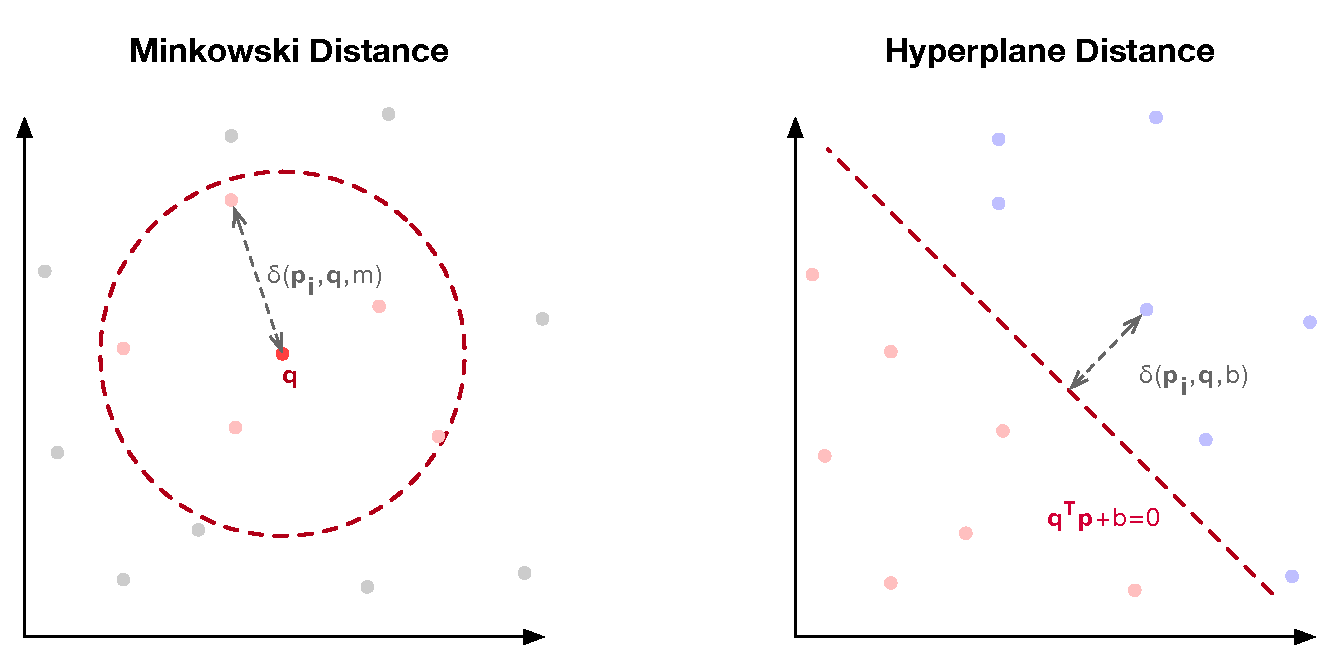
\includegraphics[width=\textwidth]{figures/distance_computations.eps}
    \caption{Two examples of distance functions that fall into the broader category of a DFC. On the left, the point-distance between $q$ and $p_i$ and on the right, the distance between a hyperplane $q^Tx+b = 0$ and points $p_i$.}
    \label{figure:distance_computation}
\end{figure}

\subsubsection{Parametrized Dimensionality}
As an aside, we must address the role of dimensionality $dim$ in the case of vector spaces such as $\mathbb{R}^{dim}$ or $\mathbb{C}^{dim}$. One could argue, that the dimensionality of such a vector space can also be seens as a parameter of the DFC. Nevertheless, we consider the dimensionality to be a structural property of the underlying data domain $\mathcal{D_q}$ and thus thightly coupled to the data type. This means, that dimensionality as well as the data type are well-defined and remain constant between queries for a given relation.

\subsection{Extending the Relational Model}

Using the definition of a DFC as provided in \cref{definition:dfc}, one can start to integrate DFCs into the relational data model. Following~\cite{Giangreco:2018thesis}, we first assume  $\mathbb{D}$ -- the set system of data domains supprted by the database -- to be extended by whatever data domain $\mathcal{D}_q$ is required. Following that recipe, a database management system can be extended to support every type of (mathematical) object that is useful for a given application, such as but not limited to $\mathbb{R}^{dim}$ or $\mathbb{C}^{dim}$. 

Using the idea of an extended projection $\pi_{\mathcal{A}}$ as defined in \cref{section:relational_data_model} and described by \cite{Garcia:2009Database}\todo{1-2 additional references}, the evaluation of a DFC can be expressed as follows.

\begin{definition}[label=definition:spf_rel]{Distance Function Classes (DFC) in Extended Projection}{}
    Let $\hat{\delta} \colon \mathcal{D}_q \times \mathcal{D}_q \times \mathcal{D}_{1} ... \times \mathcal{D}_{N-2} \to \mathbb{R}$ be a N-ary DFC and $\delta = \mathtt{IMP}(\hat{\delta})$ its implementation. Let further $\mathcal{R}$ be a relation with attribute $\mathcal{A}_p \in \mathtt{SCH}(\mathcal{R})$. The \emph{extended projection} $\pi_{\delta(\mathcal{A}_p)}(\mathcal{R})$ describes the evaluation of $\delta$ using $\mathcal{A}_p$ as probing argument. $\pi_{\delta(\mathcal{A}_p)}(\mathcal{R})$ introduces a new distance attribute $\mathcal{A}_d$, i.e., $\mathtt{SCH}(\pi_{\delta(\mathcal{A}_p), \mathcal{A}_1, ..., \mathcal{A}_n}(\mathcal{R})) = \mathtt{SCH}(\mathcal{R}) \cup \{ \mathcal{A}_d \}$
\end{definition}

The newly introduced attribute can also be renamed using known, relational operators. Obviously, the evaluation of multiple DFCs in a single, extended projection or the combination of simple attribute projection with the evaluation of DFCs are also allowed. 

The following expressions are valid examples of the extended projection on relation $\mathcal{R}$ with $\mathtt{SCH}(\mathcal{R}) = \{ \mathcal{A}_1, \mathcal{A}_2, \mathcal{A}_3, \mathcal{A}_4 \}$ and $\delta = \mathtt{IMP}(\hat{\delta})$: 

\begin{itemize}
    \item $\pi_{\delta_1(\mathcal{A}_1), \delta_2(\mathcal{A}_1)}(\mathcal{R})$: Evaluation of multiple DFCs.
    \item $\pi_{\delta_1(\mathcal{A}_1), \delta_1(\mathcal{A}_2)}(\mathcal{R})$: Evaluation of same DFC using different attributes.
    \item $\pi_{\delta(\mathcal{A}_1), \mathcal{A}_2, \mathcal{A}_4}(\mathcal{R})$: Evaluation DFC with attribute projection.
\end{itemize}

Combining the extended projection with the notion of a ranked relation $\mathcal{R^{\mathcal{O}}}$, the order operator $\tau_{\mathcal{O}}(\mathcal{R})$ and the k-selection operator $\lambda_k(\mathcal{R})$~\cite{Chengkai:2005RankSQL}, both described in \cref{section:rel_extensions}, we can now impose a sort order based on $\mathcal{A}_d$ and limit the cardinality of $\mathcal{R}^{\mathcal{O}}$. Hence, the three operators can be used to express a wide range of proximity based queries, including but not limited to NNS.

We use the example relation presented in \cref{example:rel_painting_w_features} to demonstrate the flexibility of the proposed form. The different types of queries that can be expressed through $\pi$, $\tau_{\mathcal{O}}$, $\lambda_k$ are listed in \cref{table:proximity_based_queries}.

\begin{example}[label=example:rel_painting_w_features]{Relation listing paintings with feature vectors}{}
    
    The following example relation $\mathcal{R}_{p}$ lists paintings with their title $\mathcal{A}_{t}$, the year of their creation $\mathcal{A}_{y}$ and some arbitrary feature vector $\mathcal{A}_{f}$ (we use abbreviations to keep the notation compact). Note that $\mathcal{D}_{f} \subset \mathbb{R}^{3}$.
        
    \begin{center}
        \begin{tabular}{ l || l | l | l |}
            $\mathcal{R}_{p}$ & $\mathcal{A}_{t}$  & $\mathcal{A}_{y}$  & $\mathcal{A}_{f}$ \\ 
            \hline
            \hline
            $t_1$ & Mona Lisa & 1506 & $\left\lbrack 0.0, 0.2, -1.3 \right\rbrack$ \\
            \hline
            $t_2$ & The Starry Night & 1889 & $\left\lbrack 1.0, 0.9, 2.6 \right\rbrack$ \\
            \hline
            ... & ... & ... & ... \\
            \hline
            $t_N$ & Las Meninas & 1665 & $\left\lbrack -0.5, 3.0, 0.8 \right\rbrack$ \\
            \hline
        \end{tabular}
    \end{center}
\end{example}

\begin{table}[tb]
    \centering
    \caption{Proximity based queries that can be expressed with $\pi$, $\tau_{\mathcal{O}}$, $\lambda_k$ based on the relation given in \cref{example:rel_painting_w_features} }
    \label{table:proximity_based_queries}
    \begin{tabular}{||l l r ||} 
     \hline
     Name & Result & Algebraic Form \\
     \hline\hline
     NNS / kNN & $\mathcal{R}^{ASC(\mathcal{A}_d)}$ & $\lambda_k (\tau_{ASC(\mathcal{A}_d)} ( \pi_{\mathcal{A}_{y}, \delta(\mathcal{A}_{f})}  ( \mathcal{R}_p^{\emptyset})))$  \\ 
     \hline
     FNS / kFN / MIPS & $\mathcal{R}^{DSC(\mathcal{A}_d)}$ & $\lambda_k (\tau_{DSC(\mathcal{A}_d)} ( \pi_{\mathcal{A}_{y}, \delta(\mathcal{A}_{f})}  ( \mathcal{R}_p^{\emptyset})))$   \\
     \hline
     NNS w. cut-off / $\epsilon$NN & $\mathcal{R}^{ASC(\mathcal{A}_d)}$ & $\tau_{DSC(\mathcal{A}_d)} ( \sigma_{\mathcal{A}_d \leq \epsilon} ( \pi_{\mathcal{A}_{y}, \delta(\mathcal{A}_{f})} ( \mathcal{R}_p^{\emptyset})) )$  \\
     \hline
     NNS after Selection & $\mathcal{R}^{ASC(\mathcal{A}_d)}$ &  $\tau_{DSC(\mathcal{A}_d)} ( \pi_{\mathcal{A}_{year}, \delta(\mathcal{A}_{f})} ( \sigma_{\mathcal{A}_{y} = 1889} ( \mathcal{R}_p^{\emptyset})) )$\\
     \hline
     Order by multiple features & $\mathcal{R}^{ASC(\mathcal{A}_{d1}),ASC(\mathcal{A}_{d2})}$ & \\ 
     \hline
     Aggreation on distance & $\mathcal{R}^{\emptyset}$ & \\ 
     \hline
    \end{tabular}
\end{table}


\subsubsection{Properties of $\pi$, $\tau_{\mathcal{O}}$, $\lambda_k$}

\todo[inline]{Elaborate on algebraic properties of $\pi$, $\tau_{\mathcal{O}}$, $\lambda_k$}

\subsubsection{Combination with Other Extensions}

\todo[inline]{Elaborate on how $\pi$, $\tau_{\mathcal{O}}$, $\lambda_k$ can be combined with other relational extensions}

\subsection{DFCs and Query Planning}
\label{section:dfc_and_planning}

\todo[inline]{Elaborate on how the structure of a DFC can be exploited for query planning}


\section{Cost Model for Retrieval Accuracy}
Describe cost model for execution plans with following properties:

\begin{itemize}
    \item Cost as a function of atomic costs: $f(a_{cpu}, a_{io}, a_{memory}, a_{accuracy}) \longrightarrow C$
    \item Means to estimate results accuracy and associated considerations from execution path (e.g., when using index) based on properties of the index
    \item Means to specify importance of accurate results (e.g., global, per-query, context-based i.e. when doing 1NN search) in comparison to other factors
    \item Systems perspective 1: How can such a cost model be applied during query planning and optimization?
\end{itemize}

\section{Adaptive Index Management}

\begin{figure}[h!]
    \centering
    \begin{subfigure}[b]{0.40\textwidth}
        \centering
        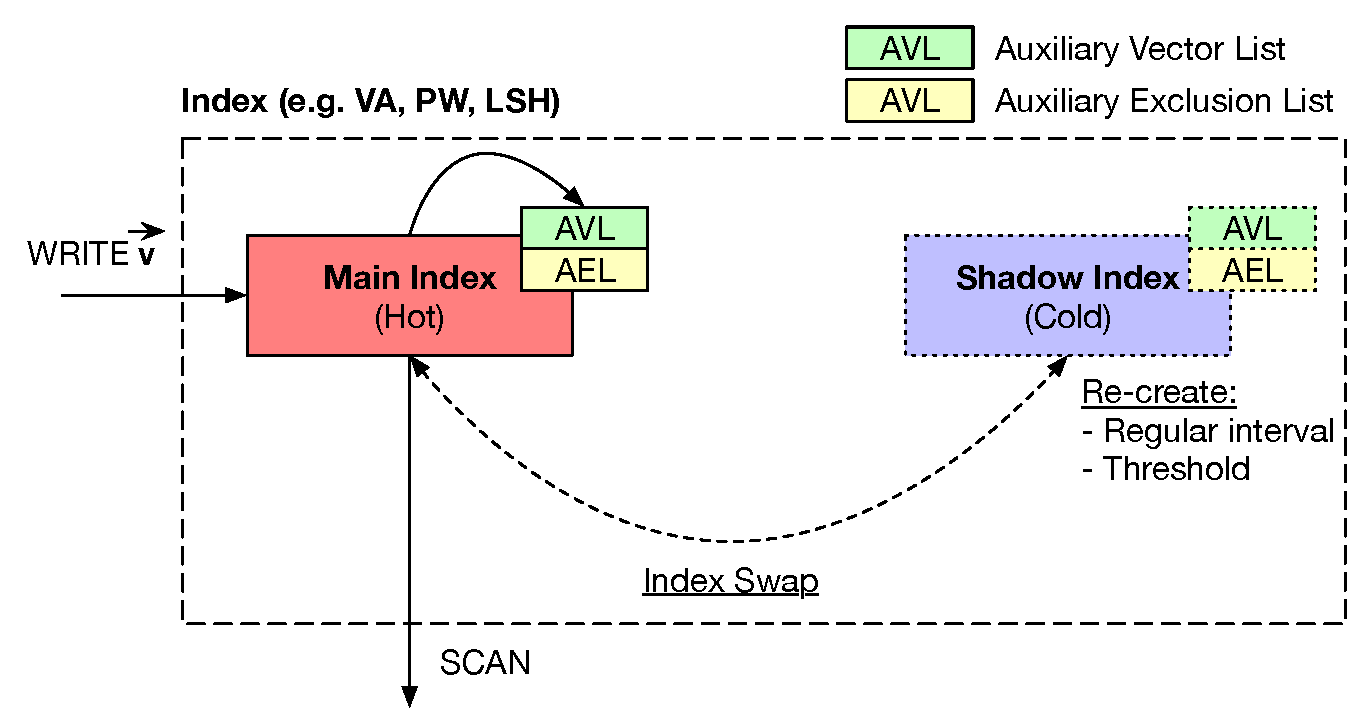
\includegraphics[width=\textwidth]{figures/adaptive_index.eps}
        \label{fig:adaptive_index:architecture}
    \end{subfigure}
    \hfill
    \begin{subfigure}[b]{0.40\textwidth}
        \centering
        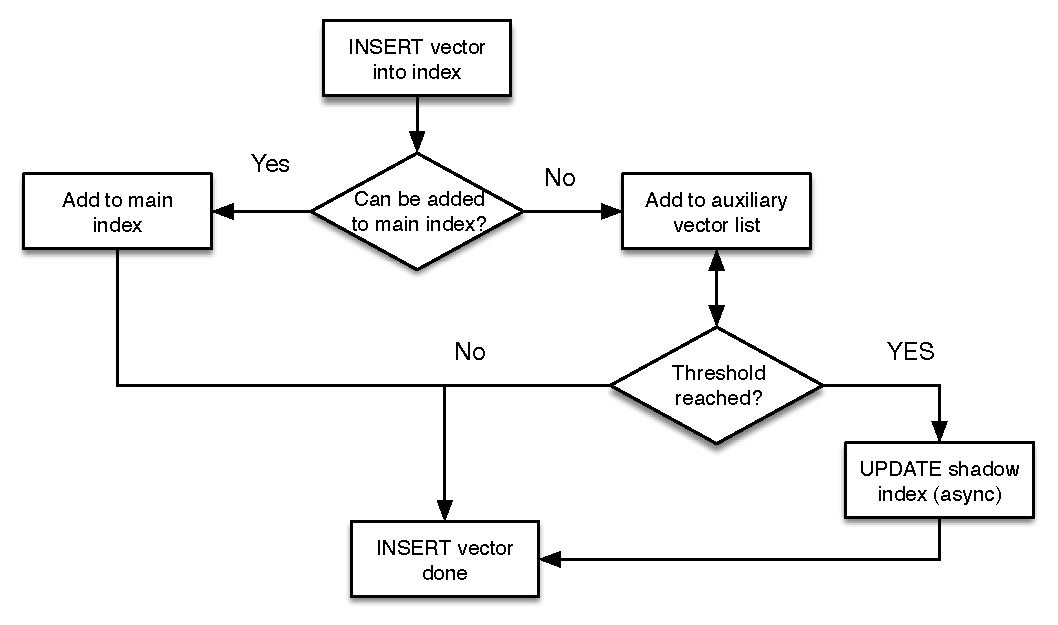
\includegraphics[width=\textwidth]{figures/adaptive_index_flow.eps}
        \label{fig:adaptive_index:flow}
    \end{subfigure}
    \caption{Adaptive index structures overview.}
    \label{fig:adaptive_index}
\end{figure}

Describe model for index management in the face of changing data (adaptive index management):

\begin{itemize}
    \item Reason about properties of secondary indexes for NNS (e.q., PQ, VA, LSH) with regards to data change
    \item Derivation of error bounds possible (e.g., usable for planning)?! Use in query planning?
    \item Systems perspective 1: How to cope with ``dirty'' indexes? Proposal: hot vs. cold index, auxilary data structure, offline optimization, see \cref{fig:adaptive_index}
    \item Systems perspective 2: On-demand index based on query workload?
\end{itemize}

\section{Architecture Model}

\todo[inline]{Putting everything together into a unified systems model (base on previous work + aforementioned aspects).}




